\documentclass[preprint,12pt,aps,pra,showkeys,amsmath,amssymb,superscriptaddress,floatfix]{revtex4-2}
\usepackage[T1]{fontenc}
\usepackage[utf8]{inputenc}
\usepackage{amsmath,amssymb,amsthm,mathtools,mathrsfs}
\usepackage{microtype,booktabs,enumitem}
\usepackage{xcolor,tikz,etoolbox}
\usepackage[skins,breakable]{tcolorbox}
\usepackage{needspace}
% Keep diagram geometry independent of REVTeX preprint body spacing.
\AtBeginEnvironment{tikzpicture}{\linespread{1}\selectfont}
\usetikzlibrary{arrows.meta,positioning,calc,fit,decorations.pathreplacing}
\usepackage{graphicx}
\usepackage{hyperref}

\definecolor{MMBlue}{RGB}{0,82,155}
\definecolor{MMOrange}{RGB}{200,80,0}
\tikzset{
 mmnode/.style={draw=MMBlue,rounded corners=2pt,fill=MMBlue!4,align=left,execute at begin node={\raggedright},text width=5cm,font=\fontsize{10}{12}\selectfont,inner sep=6pt},
 mmimport/.style={mmnode,draw=black!65,fill=black!4},
 mmcandidate/.style={mmnode,draw=MMOrange,dashed,fill=MMOrange!5},
 mmrejected/.style={mmnode,draw=black,densely dotted,fill=black!8},
 mmproof/.style={->,thick,MMBlue},
 mmflow/.style={->,semithick,black!70},
 mmrepair/.style={->,dashed,thick,MMOrange},
 mmcandidatearrow/.style={->,dashed,semithick,MMOrange},
 mmnote/.style={font=\scriptsize,fill=white,inner sep=2pt,align=center}}

\usepackage[section]{placeins}
\setlength{\emergencystretch}{3em}
\setlist{itemsep=3pt,topsep=4pt}
\newtheorem{theorem}{Theorem}[section]
\newtheorem{proposition}[theorem]{Proposition}
\newtheorem{lemma}[theorem]{Lemma}
\newtheorem{corollary}[theorem]{Corollary}
\theoremstyle{definition}
\newtheorem{definition}[theorem]{Definition}
\newtheorem{example}[theorem]{Example}
\theoremstyle{remark}
\newtheorem{remark}[theorem]{Remark}
% Avoid isolated statement headings and single-line paragraph fragments.
\BeforeBeginEnvironment{theorem}{\Needspace{6\baselineskip}}
\BeforeBeginEnvironment{definition}{\Needspace{5\baselineskip}}
\BeforeBeginEnvironment{proposition}{\Needspace{5\baselineskip}}
\BeforeBeginEnvironment{lemma}{\Needspace{5\baselineskip}}
\BeforeBeginEnvironment{corollary}{\Needspace{5\baselineskip}}
\clubpenalty=5000
\widowpenalty=5000
\newcommand{\R}{\mathbb R}\newcommand{\Z}{\mathbb Z}\newcommand{\N}{\mathbb N}
\newcommand{\Pa}{\operatorname{Pa}}\newcommand{\Desc}{\operatorname{Desc}}
\newcommand{\cl}{\operatorname{cl}}\newcommand{\cost}{\operatorname{cost}}
\newcommand{\status}{\operatorname{status}}
% Faculty cards: a visual rail groups the five faculties within one agent.
% The rail has no arrowhead and does not represent a proof dependency.
\newcommand{\mmfacultybadge}[1]{%
 \node[circle,draw=MMBlue,line width=1pt,fill=white,
 minimum size=7mm,inner sep=0pt,font=\sffamily\small\bfseries,text=MMBlue]
 at ([xshift=15pt,yshift=-15pt]frame.north west) {#1};}
\newcommand{\mmfacultyrail}{%
 \draw[MMBlue!80,line width=1pt]
 ([xshift=15pt,yshift=2pt]frame.north west)--
 ([xshift=15pt,yshift=-2pt]frame.south west);}
\newtcolorbox{mmfacultybox}[2]{enhanced,breakable,
 colback=MMBlue!4,colframe=MMBlue!4,boxrule=0pt,arc=3pt,
 left=39pt,right=9pt,top=4pt,bottom=4pt,
 before skip=2pt,after skip=2pt,
 fontupper=\small\linespread{1.1}\selectfont,
 overlay unbroken={\mmfacultyrail\mmfacultybadge{#1}},
 overlay first={\mmfacultyrail\mmfacultybadge{#1}},
 overlay middle={\mmfacultyrail},overlay last={\mmfacultyrail}}
\newcommand{\mmfaculty}[3]{%
 \begin{mmfacultybox}{#1}{#2}
 {\sffamily\bfseries\color{MMBlue}#2}\par\smallskip #3
 \end{mmfacultybox}}
\newcommand{\agent}[9]{%
 \Needspace{8\baselineskip}
 \subsubsection{#1}
 \noindent\textbf{Object.} #2\par
 \noindent\textbf{Role.} #3\par\smallskip
 \mmfaculty{E}{Ego}{#4}
 \mmfaculty{M}{Memory}{#5}
 \mmfaculty{I}{Intellect}{#6}
 \mmfaculty{S}{Sense}{#7}
 \mmfaculty{A}{Action}{#8}
 \smallskip\noindent #9\par}

\usepackage{longtable,array,calc}
\providecommand{\tightlist}{\setlength{\itemsep}{2pt}\setlength{\parskip}{0pt}}
\makeatletter
\def\frontmatter@abstract@produce{\par\addvspace{\frontmatter@preabstractspace}%
\begingroup\prep@absbox\unvbox\absbox\post@absbox\endgroup
\addvspace{\frontmatter@postabstractspace}}
\makeatother
\newcommand{\field}[2]{\par\smallskip\noindent\textbf{#1.} #2\par}
\setlength{\emergencystretch}{5em}
\AtBeginEnvironment{verbatim}{\small\linespread{1.0}\selectfont}


\hypersetup{colorlinks=true,linkcolor=MMBlue,urlcolor=MMBlue,pdfauthor={Dibakar Sigdel}}

\begin{document}

\title{Local Quadratic Convergence of Newton's Method\\[4pt]\large An End-to-End Meta-Math Walkthrough}

\author{Dibakar Sigdel}

\affiliation{Mindverse Computing LLC, Lynnwood, WA 98087, USA}

\date{October 2026}

\begin{abstract}

Express the next error as an integral of derivative differences. The
quadratic estimate then proves its own invariant neighborhood, avoiding
a circular assumption that all iterates remain near the root. The report
presents the target theorem, declared imports, a dependency graph,
five-faculty node contracts, a continuous proof, a worked example, and a
hypothesis-repair audit. It is an authored mathematical exposition, not
a deployed-agent transcript or a formal proof-assistant certificate.

\end{abstract}\maketitle\linespread{1.12}\selectfont

\noindent\textbf{ON-04 / Optimization and Numerical Analysis / Report v1}

\section{Target and import contract}

\begin{theorem}

Let \(f\) be \(C^2\) on an open interval containing
\([\alpha-r,\alpha+r]\), where \(r>0\) and \(f(\alpha)=0\). Suppose
\(|f'(x)|\ge m>0\) and \(|f''(x)|\le M\) on that closed interval, with
\(q=Mr/(2m)<1\). For every \(x_0\) in the interval, the exact Newton
iteration \(x_{k+1}=x_k-f(x_k)/f'(x_k)\) is well defined, stays in the
interval, and converges to \(\alpha\), with
\(|x_{k+1}-\alpha|\le (M/(2m))|x_k-\alpha|^2\).

\end{theorem}

\subsection{Foundations and permitted imports}

Use the fundamental theorem of calculus and its estimate
\(|f'(u)-f'(v)|\le M|u-v|\) on the interval, obtained by integrating
\(f''\). No existence of a root is inferred from numerical residuals:
the theorem assumes the root \(\alpha\) and proves convergence near it.
Every simple root has some neighborhood satisfying these hypotheses by
continuity and a sufficiently small radius.

\clearpage\section{Node interaction workflow}

\begin{center}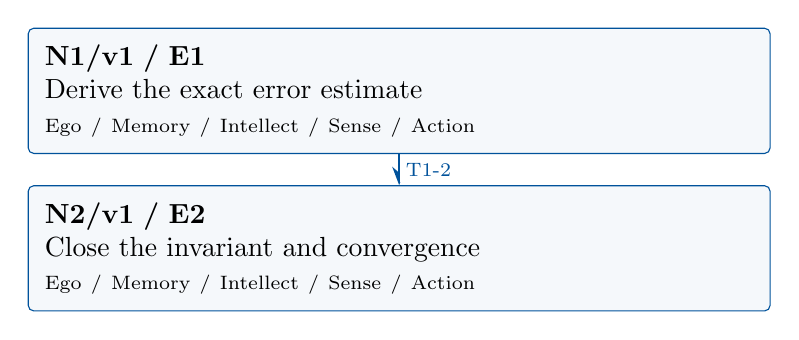
\begin{tikzpicture}[>=Stealth,x=1cm,y=1cm]

\node[mmnode,text width=9cm,minimum height=1.25cm] (N1) at (0,0.0) {\textbf{N1/v1 / E1}\\Derive the exact error estimate\\{\scriptsize Ego / Memory / Intellect / Sense / Action}};

\node[mmnode,text width=9cm,minimum height=1.25cm] (N2) at (0,-2.0) {\textbf{N2/v1 / E2}\\Close the invariant and convergence\\{\scriptsize Ego / Memory / Intellect / Sense / Action}};

\draw[mmproof] (N1.south) -- node[mmnote,right] {T1-2} (N2.north);

\end{tikzpicture}\end{center}

Each box is one mathematical agent containing all five faculties. Blue
arrows carry the versioned exports listed below. The layout gives a
reading order; only drawn arrows assert dependencies. Diagnostic repair
is separate from the proof DAG.

\subsection{Versioned evidence-transfer ledger}

\begingroup\small\linespread{1.05}\selectfont

\Needspace{5\baselineskip}\field{T1-2: N1/E1/v1 to N2}{For \(N(x)=x-f(x)/f'(x)\), \(|N(x)-\alpha|\le (M/(2m))|x-\alpha|^2\).}

\field{Receiving activity}{N2.1}

\field{Compatibility}{E1/v1 and \(q=Mr/(2m)<1\). Check: Proving the estimate at one point is
insufficient unless its next iterate stays where the hypotheses hold.}

\endgroup

\clearpage\section{Agent roles and five-faculty activities}\begingroup\small\linespread{1.05}\selectfont\setlist{itemsep=1pt,topsep=2pt}

\subsection{N1/v1: Derive the exact error estimate}

\field{Object and role}{Subtract the secant integral from the tangent term and bound the
derivative variation. \textbf{Local obligation:} For
\(N(x)=x-f(x)/f'(x)\), \(|N(x)-\alpha|\le (M/(2m))|x-\alpha|^2\).}

\field{Inputs}{\(x\in[\alpha-r,\alpha+r]\) and \(f(\alpha)=0\).}

\mmfaculty{E}{Ego}{Publish E1/v1 only after establishing this obligation: For
\(N(x)=x-f(x)/f'(x)\), \(|N(x)-\alpha|\le (M/(2m))|x-\alpha|^2\).}

\mmfaculty{M}{Memory}{\(x\in[\alpha-r,\alpha+r]\) and \(f(\alpha)=0\). Retain the stated
assumptions and import versions.}

\mmfaculty{I}{Intellect}{Subtract the secant integral from the tangent term and bound the
derivative variation.}

\mmfaculty{S}{Sense}{The denominator stays away from zero by \(m\); the entire integration
segment stays in the stated interval.}

\mmfaculty{A}{Action}{Carry out activities N1.1--N1.2 below, retaining each calculation and
construction as evidence.}

\smallskip\noindent\textbf{Numbered mathematical activities}

\begin{enumerate}[label=N1.\arabic*,leftmargin=3.4em]

\item Let \(e=x-\alpha\). The fundamental theorem gives
\(f(x)=\int_\alpha^x f'(t)\,dt\). Therefore
\(N(x)-\alpha=[e f'(x)-f(x)]/f'(x)=\bigl(\int_\alpha^x(f'(x)-f'(t))\,dt\bigr)/f'(x)\).

\item The absolute numerator is at most the integral of \(M|x-t|\) along the
segment, namely \(M|e|^2/2\). Divide by \(|f'(x)|\ge m\) to obtain the
error estimate. This remains valid for \(x<\alpha\) after taking the
absolute value of the oriented integral.

\end{enumerate}

\field{Export E1/v1}{For \(N(x)=x-f(x)/f'(x)\), \(|N(x)-\alpha|\le (M/(2m))|x-\alpha|^2\).}

\field{Acceptance gate}{The denominator stays away from zero by \(m\); the entire integration
segment stays in the stated interval.}

\field{Targeted repair}{If a Taylor remainder is used without a bound over the whole segment,
use this integral identity with the explicit uniform bound \(M\).
Withhold this export and recheck its descendants after a versioned
correction.}

\clearpage

\subsection{N2/v1: Close the invariant and convergence}

\field{Object and role}{Inductively keep every error within the radius, then sum no errors at
all: directly contract their magnitudes. \textbf{Local obligation:} All
iterates exist, \(|x_k-\alpha|\le q^k|x_0-\alpha|\to0\), and the
quadratic bound holds at every step.}

\field{Inputs}{E1/v1 and \(q=Mr/(2m)<1\). Incoming proof exports: E1/v1 at N2.1.}

\mmfaculty{E}{Ego}{Publish E2/v1 only after establishing this obligation: All iterates
exist, \(|x_k-\alpha|\le q^k|x_0-\alpha|\to0\), and the quadratic bound
holds at every step.}

\mmfaculty{M}{Memory}{E1/v1 and \(q=Mr/(2m)<1\). Incoming proof exports: E1/v1 at N2.1. Retain
the stated assumptions and import versions.}

\mmfaculty{I}{Intellect}{Inductively keep every error within the radius, then sum no errors at
all: directly contract their magnitudes.}

\mmfaculty{S}{Sense}{Proving the estimate at one point is insufficient unless its next
iterate stays where the hypotheses hold.}

\mmfaculty{A}{Action}{Carry out activities N2.1--N2.2 below, retaining each calculation and
construction as evidence.}

\smallskip\noindent\textbf{Numbered mathematical activities}

\begin{enumerate}[label=N2.\arabic*,leftmargin=3.4em]

\item If \(|x_k-\alpha|\le r\), E1 gives
\(|x_{k+1}-\alpha|\le(M/(2m))|x_k-\alpha|^2\le q|x_k-\alpha|\le qr<r\)
(with immediate equality to zero allowed). The initial point satisfies
the premise, so induction proves that every denominator is nonzero and
every iterate remains in the interval.

\item The same estimate yields \(|x_k-\alpha|\le q^k|x_0-\alpha|\), proving
convergence. At each step E1 supplies the stronger quadratic error
inequality. If \(M=0\), the first step reaches the root exactly. Finally
a simple root has \(|f'(\alpha)|>0\); continuity gives a neighborhood
with a positive derivative bound, bounded \(f''\), and after shrinking
the radius, \(q<1\).

\end{enumerate}

\field{Export E2/v1}{All iterates exist, \(|x_k-\alpha|\le q^k|x_0-\alpha|\to0\), and the
quadratic bound holds at every step.}

\field{Acceptance gate}{Proving the estimate at one point is insufficient unless its next
iterate stays where the hypotheses hold.}

\field{Targeted repair}{If local convergence is concluded while the iterates may leave the
neighborhood, choose and prove an invariant radius before repeating the
estimate. Withhold this export and recheck its descendants after a
versioned correction.}

\endgroup\clearpage\section{Continuous mathematical proof}\label{sec:proof}

\subsection{N1 --- Derive the exact error
estimate}\label{n1-derive-the-exact-error-estimate}

\begin{enumerate}
\def\labelenumi{\arabic{enumi}.}
\item
  \textbf{N1.1.} Let \(e=x-\alpha\). The fundamental theorem gives
  \(f(x)=\int_\alpha^x f'(t)\,dt\). Therefore
  \(N(x)-\alpha=[e f'(x)-f(x)]/f'(x)=\bigl(\int_\alpha^x(f'(x)-f'(t))\,dt\bigr)/f'(x)\).
\item
  \textbf{N1.2.} The absolute numerator is at most the integral of
  \(M|x-t|\) along the segment, namely \(M|e|^2/2\). Divide by
  \(|f'(x)|\ge m\) to obtain the error estimate. This remains valid for
  \(x<\alpha\) after taking the absolute value of the oriented integral.
\end{enumerate}

\subsection{N2 --- Close the invariant and
convergence}\label{n2-close-the-invariant-and-convergence}

\begin{enumerate}
\def\labelenumi{\arabic{enumi}.}
\item
  \textbf{N2.1.} If \(|x_k-\alpha|\le r\), E1 gives
  \(|x_{k+1}-\alpha|\le(M/(2m))|x_k-\alpha|^2\le q|x_k-\alpha|\le qr<r\)
  (with immediate equality to zero allowed). The initial point satisfies
  the premise, so induction proves that every denominator is nonzero and
  every iterate remains in the interval.
\item
  \textbf{N2.2.} The same estimate yields
  \(|x_k-\alpha|\le q^k|x_0-\alpha|\), proving convergence. At each step
  E1 supplies the stronger quadratic error inequality. If \(M=0\), the
  first step reaches the root exactly. Finally a simple root has
  \(|f'(\alpha)|>0\); continuity gives a neighborhood with a positive
  derivative bound, bounded \(f''\), and after shrinking the radius,
  \(q<1\).
\end{enumerate}

\hfill$\square$

\section{Worked orchestration}

For \(f(x)=x^2-2\), take \(\alpha=\sqrt2\) and \(r=1/4\). On that
interval \(|f'|\ge2(\sqrt2-1/4)>2\), so \(m=2\) is valid; \(M=2\) and
\(q=1/8\). Starting at \(x_0=3/2\) gives \(x_1=17/12\) and
\(x_2=577/408\). The exact identity
\(x_{k+1}-\sqrt2=(x_k-\sqrt2)^2/(2x_k)\) displays the quadratic
mechanism.

\subsection{Boundary and hypothesis audit}

At the multiple root of \(f(x)=x^2\), Newton gives \(x_{k+1}=x_k/2\) for
\(x_k\ne0\), only linear convergence. The derivative lower bound fails
in every neighborhood of zero. Starting far away can also break local
convergence; this theorem does not promise a global basin.

\section{Illustrative failure and repair}

The following is an authored diagnostic scenario. Changed assumptions
define a new contract; they do not retroactively prove the original
statement.

\subsection{Rejected argument, diagnosis, and correction}
\textbf{Rejected N2 claim:} the quadratic error formula proves
convergence from every initial guess. \textbf{Sense:} its constants were
established only on a fixed interval, and outside it the denominator may
vanish. \textbf{Repair:} prove the radius invariant using \(q<1\) before
iteration. This supplies the missing step for the stated local theorem;
it does not extend the theorem globally. Recheck each use of E1 along
the orbit.

\subsection{Publication and reuse}
The corrected export retains its explicit assumptions. A hypothetical
revision receives a new version, and each consuming activity is
rechecked; this scenario is not a recorded runtime event. \textbf{Next
direction:} Extend the argument to vector Newton methods using an
invertible Jacobian and a controlled inverse, with explicit matrix norm
bounds.

\par\medskip\begingroup\small\linespread{1.0}\selectfont\noindent\textbf{Provenance.} This authored proof is complete relative to its declared imports. Reuse
each export with its assumptions, proof, and version. The original
Markdown remains available for comparison.
\par\endgroup

\par\smallskip\begingroup\small\linespread{1.0}\selectfont\noindent\textbf{Further reading.} \href{https://web.stanford.edu/~boyd/cvxbook/}{Boyd and Vandenberghe,
Convex Optimization} for convexity, optimality, and descent;
\href{https://www.math.umd.edu/~mariakc/Spring2020Class.html}{University
of Maryland, Scientific Computing I} for the numerical-analysis setting.
The estimates used here are derived explicitly in §4.\par\endgroup

\end{document}
